\documentclass[ngerman,aspectratio=169,10pt]{beamer}

\usetheme[progressbar=frametitle]{metropolis}
\usepackage{appendixnumberbeamer}

\graphicspath{{./graphics/}, {./../../figures/}}

\usepackage{booktabs}
\usepackage{xspace}
\usepackage{amsmath}
\usepackage{amssymb}
\usepackage{amsthm}
\usepackage{xfrac}
\usepackage{listings}
\lstset{
	basicstyle=\ttfamily,
	showstringspaces=false,
	tabsize=4,
	upquote=true,
}

\title{Verbesserungen}
% \subtitle{}
\date{03. Februar 2021}
\author{Levin Nemesch, Joshua Sangmeister}
\institute{Algorithm Engineering - Projekt}
\titlegraphic{
    \hfill
\includegraphics[height=1.5cm]{unilogo.pdf}\\
    \hspace*{8.3cm} \textsc{AG Theoretische Informatik}
}

\begin{document}

\maketitle

\begin{frame}{ILP-Formulierung}
	\textbf{Ansätze}:
    \begin{itemize}
        \item Alternative ILP-Formulierung
        \item Alternativer exakter Algorithmus: Reduzierung auf MaxClique
        \item ILP mit neuer Separationsheuristik
        \item ILP-Formulierung mit stärkeren Constraints
    \end{itemize}
\end{frame}

\begin{frame}{Alternative ILP-Formulierung - Idee}
    Wie verhalten sich weniger, aber dafür größere Constraints?
    \begin{itemize}
        \item Laut Vorlesung nicht gut...
        \item Bisherige Formulierung: Jeder Konflikt ein Constraint
        \item Alternative: Fasse für jedes Label Konflikte zusammen
    \end{itemize}

	\begin{align*}
        && \sum_{x_{c_j}\in C_i} x_{c_j} &\leq |C_i| (1- x_i) &\forall \text{Label $i$ with $C_i$ as conflicts of i}\\
    \end{align*}

\end{frame}

\begin{frame}{Alternative ILP-Formulierung - Ergebnisse}
    \centering
    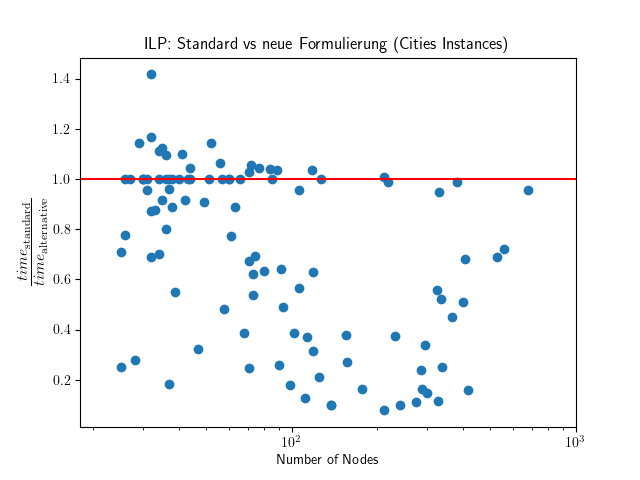
\includegraphics[width=270px]{ilp_standard_vs_alternative.png}\\
    $\longrightarrow$ Laufzeit auf mittelgroßen Instanzen schlechter, mehr Timeouts (30\%) auf größeren Instanzen
\end{frame}

\begin{frame}{Reduzierung auf MaxClique}
    \begin{itemize}
        \item Beobachtung: Optimale Lösung des Labeling-Problems bildet Clique maximaler Größe im komplementären Konfliktgraphen, da dieser Label ohne Konflikte verbindet
        \begin{itemize}
            \item Komplementärer Graph $G'$: In $G$ nicht-adjazente Knoten sind adjazent in $G'$ und umgekehrt
        \end{itemize}
        \pause
        \item Aufbauen des komplementären Konfliktgraphen, lösen mittels Maximum-Clique-Algorithmus, Rücktransformation der Lösung
        \begin{itemize}
            \item Algorithmus: MCQD, unter GNU General Public License veröffentlichte Implementation eines Papers von Konc \& Jane\^{z}i\^{c} (An improved branch and bound algorithm for the maximum clique problem, 2007)
        \end{itemize}
    \end{itemize}
\end{frame}

\begin{frame}{Reduzierung auf MaxClique}
    \begin{itemize}
        \item Als exakter Algorithmus: Gut auf kleinen Instanzen, aber extrem langsam schon auf mittleren Instanzen
        \item Bei vorzeitigem Abbruch als Heuristik verwendbar, aber auch da schlechter als Simulated Annealing oder Gurobi mit timeout
        \item Benötigt Adjazenzmatrix, Platzverbrauch macht größere Instanzen unberechenbar
    \end{itemize}
    $\longrightarrow$ Ungeeignet! Vielleicht doch lieber ILP verbessern...
\end{frame}

\begin{frame}[fragile]{ILP mit Separationsheuristik}
    \begin{itemize}
        \item Zu Beginn nur Punkt-Constraints einfügen, keine Konflikt-Constraints
        \item Separationsheuristik:
        \begin{verbatim}
sort candidates descending by number of conflicts
foreach candidate with >=1 conflict:
    find max clique in this candidates conflicts
    add cut for all members of this clique
    remove conflicts of clique from graph
    break if "enough" cuts were generated
        \end{verbatim}
    \end{itemize}
    \pause
    $\longrightarrow$ deutlich langsamer
\end{frame}

\begin{frame}{ILP mit stärkeren Constraints}
    \begin{itemize}
        \item Beobachtung 1: einfach zu ermitteln, ob Punkt in einem anderen Label liegt
        \item Beobachtung 2: wenn Punkt in Label liegt, hat dieses Konflikte mit allen Kandidaten des Punktes
    \end{itemize}
    \pause
    $\longrightarrow$ Simple Verbesserung: Bei Generierung der Punkt-Constraints direkt alle Kandidaten mit einbeziehen, die den Punkt umschließen und auf die dadurch abgedeckten paarweisen Konflikte der Label verzichten\\
    $\Longrightarrow$ stärkere Ungleichungen
\end{frame}

\begin{frame}{ILP mit stärkeren Constraints}
    \centering
    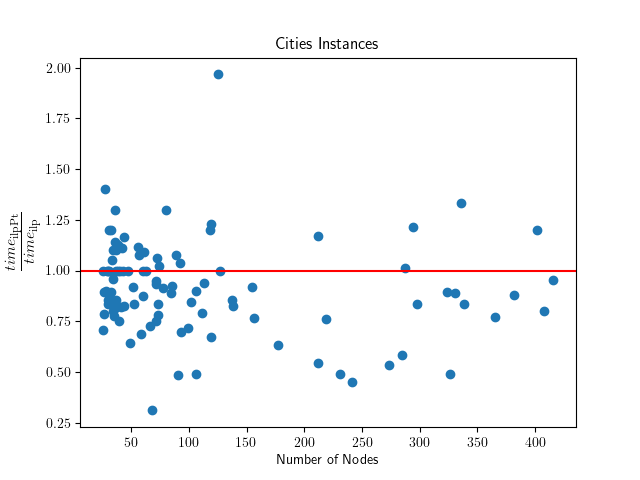
\includegraphics[width=270px]{time_ilppt_vs_ilp}\\
    Yay! Eine Verbesserung! (zumindest meistens...)
\end{frame}

\begin{frame}{ILP mit stärkeren Constraints}
    Welche Instanzen profitieren eher?
    
    \centering
    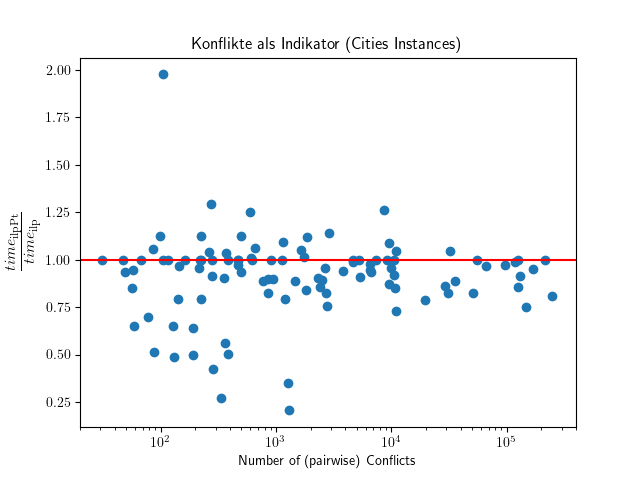
\includegraphics[width=270px]{time_vs_noConflicts}
    
\end{frame}

\end{document}